% Created 2022-10-08 Sat 15:01
% Intended LaTeX compiler: pdflatex
\documentclass[11pt]{article}
\usepackage[utf8]{inputenc}
\usepackage[T1]{fontenc}
\usepackage{graphicx}
\usepackage{grffile}
\usepackage{longtable}
\usepackage{wrapfig}
\usepackage{rotating}
\usepackage[normalem]{ulem}
\usepackage{amsmath}
\usepackage{textcomp}
\usepackage{amssymb}
\usepackage{capt-of}
\usepackage{hyperref}
\usepackage{parskip}
\author{Omkar Girish Kamath}
\date{\today}
\title{Specification Document}
\hypersetup{
 pdfauthor={Omkar Girish Kamath},
 pdftitle={Specification Document},
 pdfkeywords={},
 pdfsubject={},
 pdfcreator={Emacs 26.3 (Org mode 9.1.9)}, 
 pdflang={English}}
\begin{document}

\maketitle
\tableofcontents

\section{Modules in the processor}
\label{sec:orga7cb9c0}
\subsection{RAM}
\label{sec:orga8fe5ad}
\subsubsection{Theory}
\label{sec:org753cf2b}
\subsubsection{Interface}
\label{sec:org899eb12}
\subsection{Program Counter}
\label{sec:org4995f51}
\subsubsection{Theory}
\label{sec:org913cfa5}
\begin{figure}[htbp]
\centering
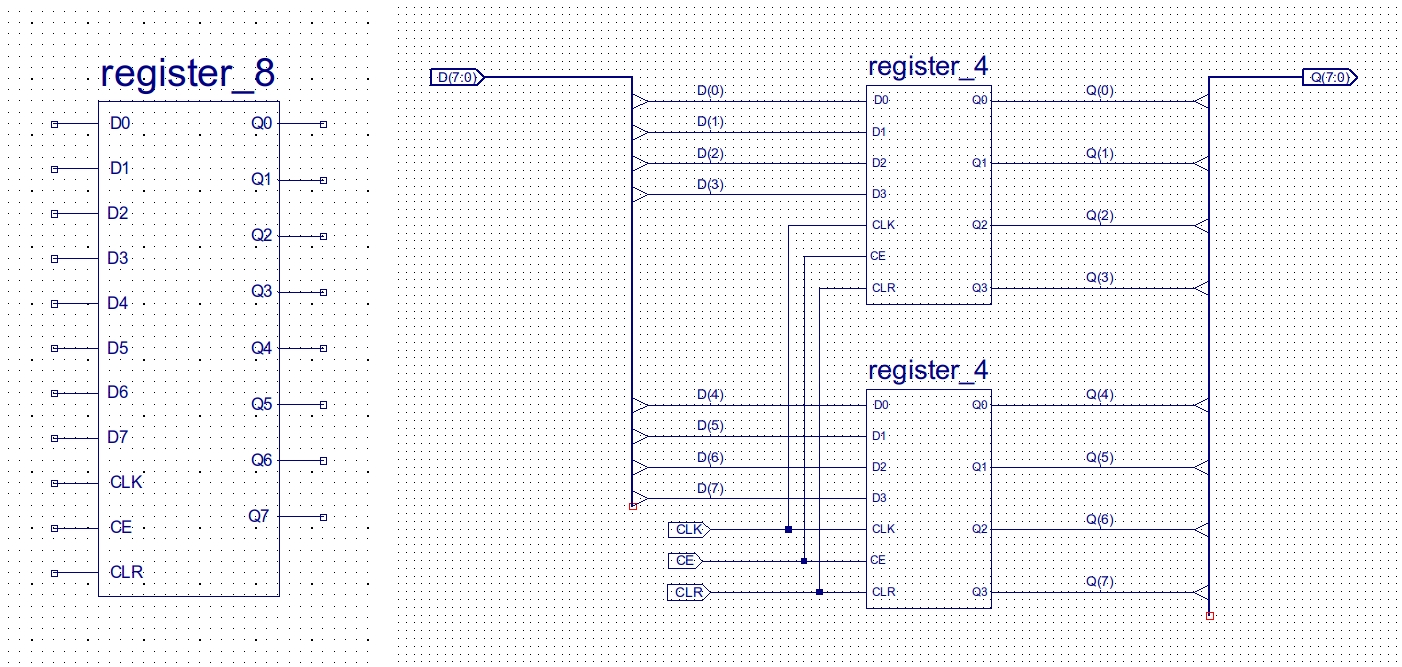
\includegraphics[width=.9\linewidth]{./images/reg8.jpg}
\caption{\label{fig:org85e7ab1}
}
\end{figure}
8 bit register used to store the address \textbf{current} instruction being executed.
It is incremented after every \emph{fetch-decode-execute-increment} cycle .
\subsubsection{Interface}
\label{sec:org4b00782}
module pc (\\
d,\\
clk,\\
ce,\\
clr,\\
q\\
);

input [7:0] d     ; \\
input clk         ;   \\
input ce      ; \\
input clr     ; \\
output [7:0 ]q; \\

\begin{center}
\begin{tabular}{lll}
signal name & type & size\\
\hline
d & input & 8 bits\\
clk & input & 1 bit\\
ce & input & 1 bit\\
clr & input & 1 bit\\
q & output & 8 bits\\
 &  & \\
\hline
\end{tabular}
\end{center}
\subsection{Instruction Register}
\label{sec:orgd72ce65}
\subsubsection{Theory}
\label{sec:org948ceb0}
Instruction Register (IR) : \textbf{16} bit register, updated at the end of the fetch phase with the instruction to be processed (decoded and executed).
\begin{center}
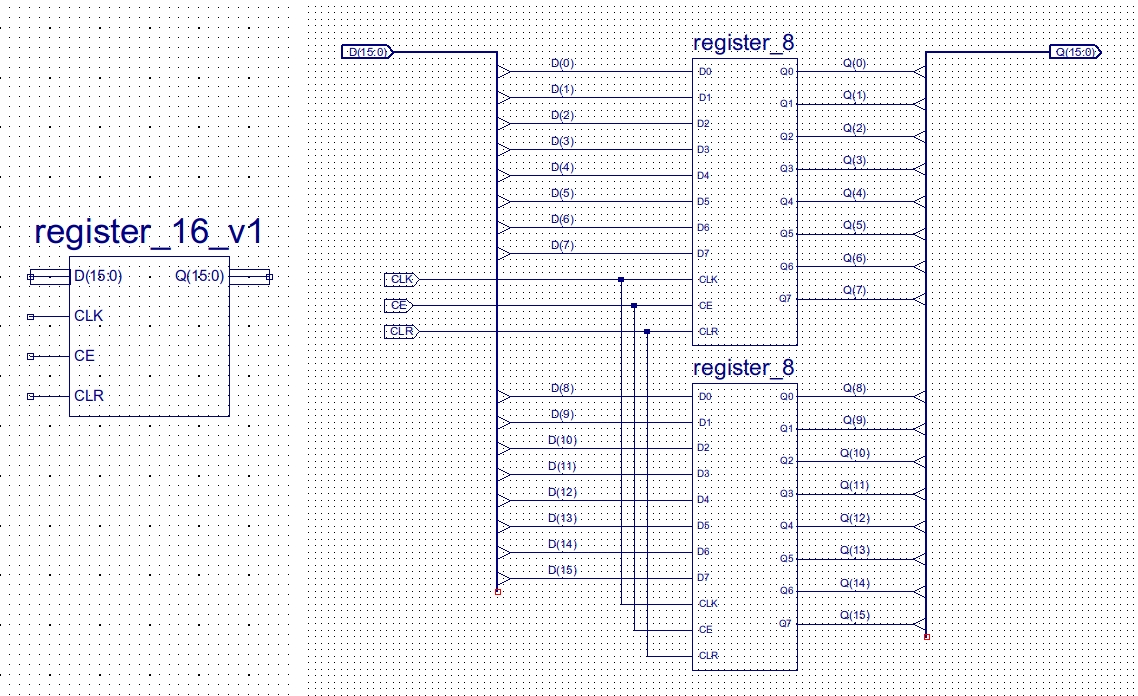
\includegraphics[width=.9\linewidth]{./images/reg16.jpg}
\end{center}
\subsubsection{Interface}
\label{sec:org551ce80}
module ir (\\
    d,\\
    clk,\\
    ce,\\
    clr,\\
    q\\
    );\\

input  [15:0] d     ; \\
input         clk   ;   \\
input         ce    ; \\
input         clr   ; \\
output [15:0] q     ; \\

\begin{center}
\begin{tabular}{lll}
signal name & type & size\\
\hline
d & input & 16 bits\\
clk & input & 1 bit\\
ce & input & 1 bit\\
clr & input & 1 bit\\
q & output & 16 bits\\
\hline
\end{tabular}
\end{center}

\subsection{Decoder}
\label{sec:org5e2d5c1}
\subsubsection{Theory}
\label{sec:org55d233d}

\subsubsection{Interface}
\label{sec:orgb9093a0}
\begin{center}
\begin{tabular}{lrll}
Name & size & function & type\\
\hline
mux\(_{\text{a}}\) & 1 & ALU A input MUX control & output\\
mux\(_{\text{b}}\) & 1 & ALU B input MUX control & output\\
mux\(_{\text{c}}\) & 1 & address MUX control, selecting PC or IR & output\\
en\(_{\text{da}}\) & 1 & accumulator (ACC) register update control & output\\
en\(_{\text{pc}}\) & 1 & program counter (PC) register update control & output\\
en\(_{\text{ir}}\) & 1 & instruction register (IR) update control & output\\
ram\(_{\text{we}}\) & 1 & memory write enable control & output\\
alu\(_{\text{c}}\) & 5 & ALU control line & output\\
ir & 8 & high byte of instruction register, contains opcode & input\\
zero & 1 & connected to ALU output, if 1 indicates result is zero & output\\
clk & 1 & system clock & input\\
ce & 1 & clock enable, normally set to 1, if set to 0 processor will HALT & input\\
clr & 1 & system reset, if pulsed high system will be reset & input\\
\hline
\end{tabular}
\end{center}


MUX\(_{\text{A}}\) : output, ALU A input MUX control

MUX\(_{\text{B}}\) : output, ALU B input MUX control 

MUX\(_{\text{C}}\) : output, address MUX control, selecting PC or IR 

EN\(_{\text{DA}}\) : output, accumulator (ACC) register update control 

EN\(_{\text{PC}}\) : output, program counter (PC) register update control 

EN\(_{\text{IR}}\) : output, instruction register (IR) update control 

RAM\(_{\text{WE}}\) : output, memory write enable control 

ALU\(_{\text{S0}}\) : output, ALU control line 

ALU\(_{\text{S1}}\) : output, ALU control line

ALU\(_{\text{S2}}\) : output, ALU control line 

ALU\(_{\text{S3}}\) : output, ALU control line 

ALU\(_{\text{S4}}\) : output, ALU control line 
 (\textbf{combining all the ALU control lines we get a 5 bit out alu\(_{\text{c}}\) signal}) 

IR : input bus, 8bits, high byte of instruction register, contains opcode 

ZERO : input, driven by 8bit NOR gate connected to ALU output, if 1 indicates result is zero 

CARRY : input, driven by carry out (Cout) of ALU 

CLK : input, system clock 

CE : input, clock enable, normally set to 1, if set to 0 processor will HALT 

CLR : input, system reset, if pulsed high system will be reset 

\subsection{Accumulator}
\label{sec:orgf0d36bf}
\subsubsection{Theory}
\label{sec:org97d4bcd}
\begin{figure}[htbp]
\centering
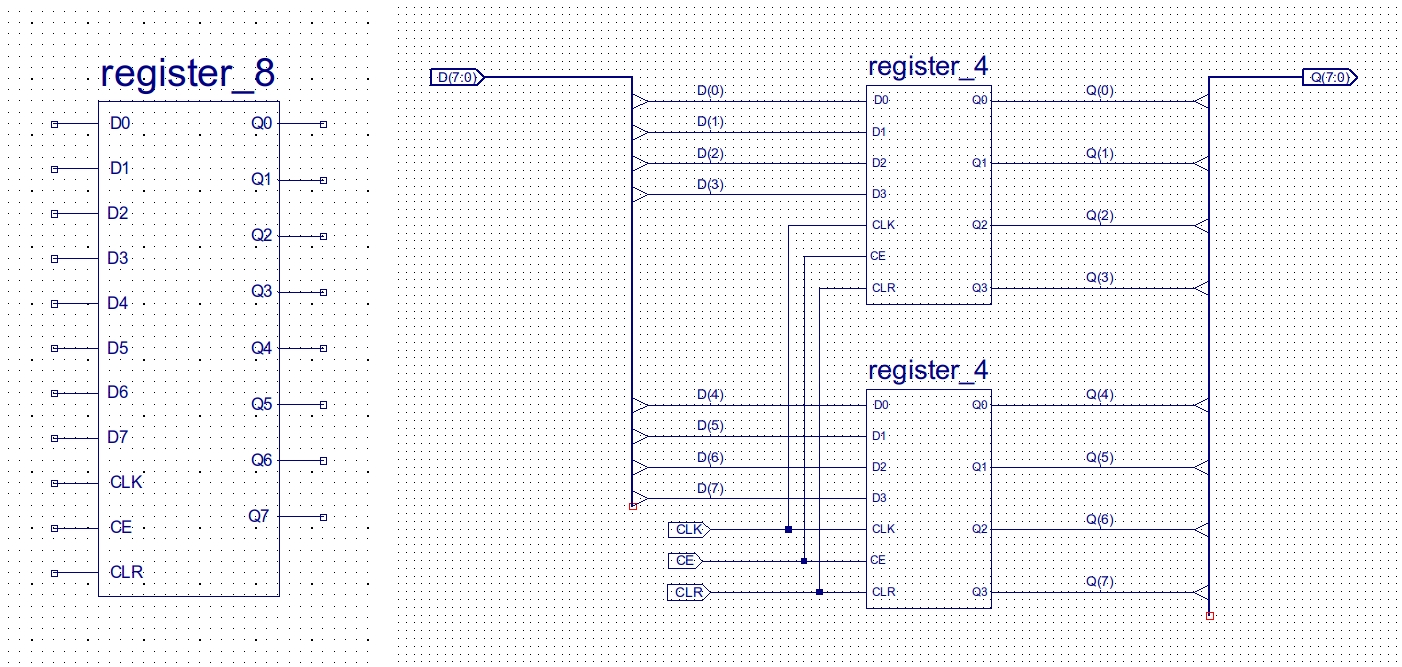
\includegraphics[width=.9\linewidth]{./images/reg8.jpg}
\caption{\label{fig:org667cddb}
}
\end{figure}
Accumulator (ACC) : \emph{8} bit register, a general purpose data register, providing data (operand) to be processed by the ALU and used to \textbf{store} any result produced. Note, we can only store one 8 bit value at a time on the processor, other data values will need to be buffered in external memory.
\subsubsection{Interface}
\label{sec:org5380740}
module pc (\\
d,\\
clk,\\
ce,\\
clr,\\
q\\
);

input [7:0] d     ; \\
input clk         ;   \\
input ce      ; \\
input clr     ; \\
output [7:0 ]q; \\

\begin{center}
\begin{tabular}{lll}
signal name & type & size\\
\hline
d & input & 8 bits\\
clk & input & 1 bit\\
ce & input & 1 bit\\
clr & input & 1 bit\\
q & output & 8 bits\\
 &  & \\
\hline
\end{tabular}
\end{center}
\subsection{ALU}
\label{sec:orgd055cb4}
\subsubsection{Theory}
\label{sec:org73722d3}
\subsubsection{Interface}
\label{sec:org1a86bf6}
\subsection{MUX}
\label{sec:orgd307ce5}
\subsubsection{MUX\(_{\text{IR to ALU}}\)}
\label{sec:org6d9e60c}
\subsubsection{MUX\(_{\text{PC to ALU}}\)}
\label{sec:orgc85ba89}
\subsubsection{MUX\(_{\text{Address in RAM}}\)}
\label{sec:org43d153d}
\end{document}
